%% naoimi.tex
%% Mac Radigan
\documentclass{article}[11pt]
%\documentclass{report}
\setcounter{secnumdepth}{7}
%\usepackage{draftcopy}
\usepackage[framed,numbered,autolinebreaks,useliterate]{mcode}
\usepackage{setspace}
\usepackage[left=1in,top=1in,right=1in,bottom=1in,nohead]{geometry}
\usepackage{graphicx,amssymb,amstext,amsmath,amsthm,caption,mathtools}
\usepackage{algorithm}
\usepackage{algorithmic}
\usepackage{amsfonts}
\usepackage{amssymb}
\usepackage{csvtools}
\usepackage{pdftexcmds}
\usepackage{listing}
%\usepackage{minted}
\usepackage{fancyvrb}
\usepackage{hyperref}
\usepackage{algpseudocode}
%\usepackage{epigraph}
%\usepackage[noend]{algpseudocode}
\hypersetup{
 colorlinks,
 citecolor=blue,
 filecolor=blue,
 linkcolor=blue,
 urlcolor=blue
}
\usepackage{titlesec}
%\titleformat{\section}[block]{\Large\bfseries\filcenter}{}{}{}
%\titleformat{\section}[block]{\Large\bfseries\filcenter}{}{1em}{}
\bibliographystyle{IEEEtran}
\newcommand\Quote[1]{\lq\textsl{#1}\rq}
\newcommand\fr[2]{{\textstyle\frac{#1}{#2}}}
\newcommand{\ssection}[1]{\section[#1]{\centering\normalfont\scshape #1}}
\newcommand{\ssubsection}[1]{\subsection[#1]{\raggedright\normalfont\itshape #1}}
%\addto{\normalsize}{\setlength{\abovedisplayskip}{20ex}}

\begin{document}

\title{Normalized Algorithm Object Messaging Interface (NAOMI)}
\author{Mac Radigan}
\date{} % comment this out if you would like to include the date
\doublespacing

\maketitle

%\begin{abstract}\centering
%\end{abstract}

\begin{figure}[h]
\begin{center}
\resizebox{5in}{!}{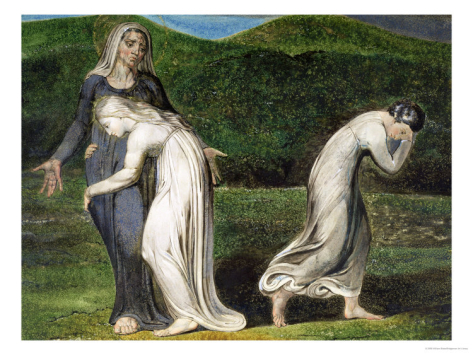
\includegraphics{images/naomi.eps}}
\end{center}
\label{fig:naomi}
\end{figure}
\newline
\newpage


\tableofcontents
%\listofalgorithms
%\listoffigures
\newpage

\section{Some Advice From Richard Hamming}

$\ldots$I was solving one problem after another after another; a fair number were successful and there were a few failures. I went home one Friday after finishing a problem, and curiously enough I wasn't happy; I was depressed. I could see life being a long sequence of one problem after another after another. After quite a while of thinking I decided, "No, I should be in the mass production of a variable product. I should be concerned with all of next year's problems, not just the one in front of my face." By changing the question I still got the same kind of results or better, but I changed things and did important work. I attacked the major problem - How do I conquer machines and do all of next year's problems when I don't know what they are going to be? How do I prepare for it? How do I do this one so I'll be on top of it? How do I obey Newton's rule? He said, "If I have seen further than others, it is because I've stood on the shoulders of giants." These days we stand on each other's feet!
\par
You should do your job in such a fashion that others can build on top of it, so they will indeed say, "Yes, I've stood on so and so's shoulders and I saw further." The essence of science is cumulative. By changing a problem slightly you can often do great work rather than merely good work. Instead of attacking isolated problems, I made the resolution that I would never again solve an isolated problem except as characteristic of a class.
\par
Now if you are much of a mathematician you know that the effort to generalize often means that the solution is simple. Often by stopping and saying, "This is the problem he wants but this is characteristic of so and so. Yes, I can attack the whole class with a far superior method than the particular one because I was earlier embedded in needless detail." The business of abstraction frequently makes things simple$\ldots$ $\mathbb{-$\mbox{ }$Richard$\mbox{ }$Hamming}$

\section{Introduction}

\par
The Normalized Algorithm Object Messaging Interface (NAOMI) is a design specification for simplifying Service-Oriented Architecture (SOA) development.

\par
The NAOMI architecture utilizes the following design practices:
\begin{itemize}
  \item Software Component Interfaces
  \item Lean POJO
  \item OSGi (JSR-291)
  \item $\mu$-Services
  \item RESTful Web Services
  \item Single Source Of Truth (SSOT)
  \item Atomic Operations (JSR-166)
  \item Functional Programming
  \item Identity, State, and Values (Rich Hickey)
  \item Continuous Integration (Karaf dev:watch with Nexus)
  \item Maven Integration and Provisioning (SpringSource DM)
  \item Lifecycle Management (Airies Blueprint)
  \item Unit Testing
  \item Dependency Injection Patterns
  \item Functional Mock-up Patterns
\end{itemize}

\section{Overview of NAOMI}

\par
The NAOMI specification provides the following for Rapid Application Development (RAD) in a SOA:
\begin{itemize}
  \item Normalized Algorithm Object Messaging Interface (NAOMI)
    \begin{itemize}
      \item parent container for all subprojects (below)
      \item flexible design can be integrated into a variety of existing architectures:
      \begin{itemize}
        \item OSGi service
        \item Java library
        \item Standalone executable JAR
        \item Script interpreter
      \end{itemize}
      \item SSH console administration and built-in logging facility (OSGi only)
      \item Lifecycle management (built-in, but improves with OSGi)
      \item Continuous Development (built-in, but improves with OSGi)
      \item Provisioning (built-in, but improves with OSGi)
    \end{itemize}
  \item Resource-Oriented Algorithm Repository (ROAR)
    \begin{itemize}
      \item RESTful webservice interface to NAOMI
      \item single repository for interface definitions
      \item updated dynamically from Maven without service interruption
      \item user-friendly XHTML interface (by XSLT from XML) 
      \item all reporting and transactions controllable through HTTP methods (URLs) using any web client or browser (by RESTful nature)
      \item provides view on software configuration and operation
    \end{itemize}
  \item Workflow Unified as a single Matrix for Processing Unlimited Services (WUMPUS)
    \begin{itemize}
      \item workflow engine based on basic network graph theory
      \item all configuration stored as a single, 2-D matrix
      \item network graph constructed automatically from software component interfaces
      \item workflow execution with concurrent atomic execution
      \item each workflow is also a 2-D matrix (submatrix)
      \item cannonical form provides a unique workflow hashcode ("normalized")
      \item RESTful interface provided by ROAR
      \item tools provided for both static and dynamic analysis
      \item access to internal matrix provided in m-file and HDF5 format
    \end{itemize}
  \item Now Yet ANother Control Algorithm Tool (NYANCAT)
    \begin{itemize}
      \item library of analysis tools for reporting and logging
      \item RESTful interface provided by ROAR
      \item provides converters from WUMPUS matrix to a variety of formats ( HTML, JPG, XML, XSL, XSD, HDF5, m-file, ...)
      \item allows for runtime and log analytics of processing
    \end{itemize}
  \item Robust Universal Test Harness (RUTH)
    \begin{itemize}
      \item test facility for unit, thread, and regression tests
      \item RESTful interface provided by ROAR
      \item automatic execution of uploaded (scriptable) test plans
      \item automatic simulation available in the absence of functional services
      \item all actions and report accessible via URL (RESTful)
      \item user-friendly XHTML interface
      \item reporting and analytics provided by NYCANCAT
    \end{itemize}
\end{itemize}


\section{NAOMI Architecture}
\subsection{Architectural Diagram}

\section{Normalized Algorithm Components}

\subsection{Resource-Oriented Algorithm Repository (ROAR)}

\par 
Resource-Oriented Algorithm Repository (ROAR) is an extensible, RESTful interface to the NAOMI system.

\par 
Updates may be installed from Maven with provisioning, and can be dynamically from Maven without service interruption (using Karaf dev:watch).

\par 
A variety of views on the both the configuration and running system are available from any web browser or HTTP client.


\subsection{Workflow Unified as a single Matrix for Processing Unlimited Services (WUMPUS)}

\par 
Workflow Unified as a single Matrix for Processing Unlimited Services (WUMPUS) provides a simple workflow engine based on basic graph theory from any undergraduate computer science curriculum.  The internal configuration may be represented by a single matrix, in particular, an oriented incident matrix with degree.  From this matrix, derivations may be made that satisfy all other graph theory needs.

\par 
By writing this configuration in cannonical form (normalized), the unique software configuration may be written as a single number (hashcode).  This number uniquely represents the system, and may be independently verified during static analysis.

\par 
The system configuration is specified by function interfaces representing each service in the SOA (functors).  The functor implementations themselves are calls to the individual services.  This function signature looks like a C-style function prototype that we are familiar with.  Parameters are further annotated additional metadata needed for the particular system.  This list of functors is the only information that is needed to construct the workflow-defining matrix.

\par 
In the absence of absence of functional services, a built-in simulator or custom simulator may be used (see RUTH).

\begin{figure}[h]
\begin{center}
\resizebox{0.5in}{!}{
\includegraphics{images/wumpus.eps}}
\end{center}
\caption{WUMPUS on day good day}
\label{fig:wumpus}
\end{figure}

\subsection{Now Yet ANother Control Algorithm Tool (NYANCAT)}

\par Now Yet ANother Control Algorithm Tool (NYANCAT) is a software tool for accessing WUMPUS configuration and processing, as well as RUTH test plans and processing logs.

\par The NYCANCAT library contains a rich set of converters for converting this data into a variety of formats:
\begin{itemize}
  \item XHTML (with MathJax)
  \item Markdown
  \item ASCII text
  \item HDF5
  \item m-file
  \item GIF, JPEG, PNG, TIF
  \item XML
  \item XSL
  \item XML Schema
\end{itemize}

\par These results are accessible via commandline, as well as through the RESTful ROAR service.

\begin{figure}[h]
\begin{center}
\resizebox{1in}{!}{
\includegraphics{images/nyancat.eps}}
\end{center}
\caption{NYANCAT on any given day}
\label{fig:nyancat}
\end{figure}

\subsection{Robust Universal Test Harness (RUTH)}

\par Robust Universal Test Harness (RUTH) is a facility for unit, thread, and regression testing.  It allows for these tests to be scripted and run automatically.  

\par The tests are recorded using RUTH's logging facility, and analytics provide detailed a detailed summary and rich graphical reporting of the historical results.

\section{Summary}

%\newpage
%\bibliography{IEEEabrv,bibliography}

\end{document}
%% *EOF*
